\documentclass{article}

\usepackage{graphicx}         % Pacote para usar os gráficos

\begin{document}

  % Na hora podemos usar qualquer imagem em vez desse pdf que eu usei
  % É importante dizer que existe uma lista de formatos aceitos (de PNG à PDF)
  \begin{figure}[h]
    \centering
    \includegraphics[scale=0.5]{abntex2-modelo-img-grafico}
    % Coloquei uma imagem (a mesma) dentro da pasta img apenas para mostrar que a imagem NÃO precisa estar obrigatoriamente na mesma pasta
    % Aí o comando ficaria assim
    % \includegraphics[scale=0.5]{img/abntex2-modelo-img-grafico} 
    \caption{Minha figura top}
    \label{fig:top}
  \end{figure}


\end{document}
